%% LyX 2.0.6 created this file.  For more info, see http://www.lyx.org/.
%% Do not edit unless you really know what you are doing.
\documentclass[english,journal=jpcafh,manuscript=article,maxauthors=0]{achemso}
\usepackage[T1]{fontenc}
\usepackage{amsmath}
\usepackage{amssymb}
\usepackage{graphicx}
\usepackage{esint}

\makeatletter

%%%%%%%%%%%%%%%%%%%%%%%%%%%%%% LyX specific LaTeX commands.

\title{Uranyl solvation by a three-dimensional reference interaction site
model}
\author{Alexei Matveev}
\email{alexei.matveev@gmail.com}
\author{Bo Li}
\author{Notker R�sch}
\email{roesch@mytum.de}
\affiliation{Department Chemie, Technische Universit�t M�nchen, 85747 Garching,
Germany}
\alsoaffiliation{Catalysis Research Center, Technische Universit�t M�nchen, 85747
Garching, Germany}
\alsoaffiliation{Institute of High Performance Computing, Agency for Science, Technology
and Research, 1 Fusionopolis Way, Connexis \#16-16, Singapore 138632,
Singapore}
%% Because html converters don't know tabularnewline
\providecommand{\tabularnewline}{\\}


%%%%%%%%%%%%%%%%%%%%%%%%%%%%%% User specified LaTeX commands.
\usepackage{mathptmx}
\usepackage{times}
%\usepackage{microtype}
%\def\thetable{\arabic{table}}
%\usepackage{ragged2e}
%\usepackage[textfont=it]{caption}
\captionsetup{font={bf}}

\makeatother

\usepackage{babel}
\begin{document}
\begin{abstract}
We report an implementation of the three-dimensional reference interaction
site model (3D RISM) that in particular addresses the treatment of
the long-range Coulomb field of charged species, represented by point
charges and/or a distributed charge density. A comparison of 1D and
3D results for atomic ions demonstrates a reasonable accuracy, even
for a moderate size of the unit cell and a moderate grid resolution.
In an application to uranyl complexes with 4\textendash{}6 explicit
aqua ligands and an implicit bulk solvent modeled by RISM, we show
that the 3D technique is not susceptible to the deficiencies of the
1D technique exposed in our previous work {[}Li, Matveev, Kr�ger,
R�sch, \emph{Comp. Theor. Chem.} \textbf{1051}, p.~151, (2015){]}.
The 3D method eliminates the artificial superposition of explicit
aqua ligands and the RISM medium and predicts essentially the same
values for uranyl and uranyl-water bond lengths as a state-of-the-art
polarizable continuum model. With the first solvation shell treated
explicitly, the observables are nearly independent of the order of
the closure relationship used when solving the set of integral equations
for the various distribution functions. Furthermore, we calculated
the activation barrier of water exchange with a hybrid approach that
combines the 3D RISM model for the bulk aqueous solvent and a quantum
mechanical description (at the level of electronic Density Functional
Theory) of uranyl interacting with explicitly represented water molecules.
The calculated result agrees very well with experiment and the best
theoretical estimates. 
\end{abstract}
\maketitle

\section{Introduction}

Thermodynamic and structural properties of the uranyl(VI) cation,
UO$_{2}^{2+}$, the most common uranium species in aqueous solution,
are crucial for understanding its environmental chemistry as well
as chemical processes in radioactive waste disposal and recycling
of used nuclear fuel \citep{book:Morss06,book:Grenthe92,Silva95}.
Simulations on the basis of quantum mechanics (QM) or classical molecular
mechanics (MM) provide two complimentary ways of addressing the microscopic
structure and the energetics of solvated uranyl species. Till now,
the most popular strategy for combining the accuracy of QM methods
and the complexity of the statistical solvent description is to apply
a polarizable continuum model (PCM) to represent the effective electrostatic
field of the solvent, usually employed in combination with phenomenological
corrections (largely relying on empirical parameters) for dispersion-repulsion
interactions and the cavity formation energy \citep{Tomasi05,Fuchs02}.
The conductor-like screening model (COSMO) of electrostatic interactions
is a state-of-the-art PCM \citep{Klamt95}; it was successfully applied
in various studies of uranyl complexes \citep{Fuchs02,Moskaleva04,Cao05,Shamov05,Gutowski06}.
On the other hand, significant efforts are being made on improving
the empirical model potentials for MM simulations, be it molecular
dynamics (MD) or Monte-Carlo (MC) methods, that yield the most explicit
statistical description of the solvent \citep{Guilbaud93,Guilbaud96,Rai12,Pomogaev13,Kerisit13,Tiwari14,book:Griebel07}.
Although several studies \citep{Gordon00,hagberg05,Frick09,Tirler13}
attempted to combine QM and stochastic MM models, such combinations
will inevitably lack the precise reproducibility and the efficiency
of analytic continuum models due to statistical sampling techniques.
More demanding QM dynamic simulations \citep{Buehl05,Buehl06,Buehl11,Nichols08}
are restricted to comparably small numbers of solvent molecules. 

Alternatively, the integral equation theories of molecular liquids
\citep{book:Hirata03,book:Hansen06} may provide sufficient accuracy
at an affordable cost for simulating chemical processes in solution
by employing standard numerical methods on contemporary hardware.
Two variants of this type are the reference interaction site model
(RISM) \citep{Chandler72,Hirata81,Hirata82,Kinoshita97} and its three-dimensional
generalization (3D RISM) \citep{Beglov95,Kovalenko98}. These methods
provide the solvent structure in form of site-site radial distribution
functions (RDFs) or three-dimensional distribution functions of solvent
sites in an external (solute) field, respectively. Both 1D and 3D
methods offer variational expressions for the solvation energy in
the form of the excess chemical potential for several types of closure
of the hierarchy of equations \citep{Singer85,Kast08}, hence admit
intuitive expressions for the first-order derivatives with respect
to nuclear displacements. For another class of integral equations
based on the Born--Green--Yvon hierarchy \citep{Fischer80,Griebel08}
the lack of a practical free energy expression complicates exploring
free energy landscapes. Note that the dielectrically consistent RISM
(DRISM) \citep{Perkyns92} is able to compensate the error of the
gas-like dielectric response of standard RISM for electrolytes and
ionic solutes \citep{Perkyns94,Chiodo07,Chuev08,Joung13}.

Handling correctly the electrostatic field of a charge distribution
requires additional care when periodic boundary conditions are employed
to simulate finite systems \citep{Makov95}. It was understood early
on that the long-range asymptotes of the radial correlation functions
induced by Coulomb interactions in RISM need a separate treatment
as well \citep{Ng74}. The few practical approaches to 3D RISM pursue
various strategies, e.g.\ inclusion of a background charge correction
\citep{Kovalenko00b}, monopole correction \citep{Kloss08b}, and
an exact re-summation for a superposition of Gaussian-type charge
distributions \citep{Perkyns10}. Very recently, a new efficient technique
has been presented to avoid integrating in real space the long-range
contributions to the solvation energy \citep{Heil15}. In this work
we present a generalization of the exact re-summation technique for
arbitrary solute charge densities.

The integral equation theory has been combined with Hartree--Fock
electronic structure theory for self-consistent field calculations
(RISM SCF) in the pioneering work of Ten-no, Hirata, and Kato who
first applied the method to formaldehyde and carbonyl compounds in
water \citep{Tenno93,Tenno94}. An extension to 3D RISM SCF was developed
for density functional theory (DFT) \citep{Kovalenko99} and \emph{ab
initio} calculations \citep{Kloss08}. Analytic energy gradients with
respect to nuclear displacements for the self-consistent combination
of DFT and 3D RISM \citep{Gusarov06} simplify exploring free energy
landscapes of complex molecular systems. Some of the recent developments
of hybrid approaches combining integral equation theories and quantum
chemistry have been discussed in a recent review \citep{Sato13}. 

In this work, we first describe our implementation of the 3D RISM
approach as well as a numerical treatment of the long-range Coulomb
field of a charged solute. Then we
validate the implementation by comparing the results of 1D and 3D
techniques for alkali and halide ions.
We further evaluate the performance of the method for the uranyl(VI)
dication in aqueous solution, represented by aqua complexes $[\text{UO}_{2}(\text{H}_{2}\text{O})_{n}]^{2+}$,
($n=4-6$), using a force field description,
and a quantum mechanical representation of the interactions within
the first solvation shell. We also compare
the results to those of PCM calculations. Finally, we analyze the
activation barrier for exchanging a water molecule in the first solvation
shell, using QM and MM models
of interactions. With the exception of the water exchange process
the test cases used to evaluate the 3D RISM approach are the same
as in our preceding work on 1D RISM \citep{Bo15}. 


\section{Methodology \label{sec:methodology}}


\subsection{3D RISM equations}

In the 3D RISM approach, the solvent sites are exposed to an external
field of a solute of general shape. The solute-solvent interactions
are assumed to be pairwise, which in the present formulation excludes
\emph{polarizable} solutes.  Furthermore, the interactions are usually
approximated by superposition of pairwise site-site contributions.
The 3D RISM equations operating with site-specific distributions can
be written as follows \citep{book:Hirata03}:

\begin{equation}
\begin{cases}
h=\chi\ast c\\
h=c+t\\
h=f(-v+t)
\end{cases}\label{eq:rsim-h-c-t}
\end{equation}
Here $h$, $c$, and $t$ are the vectors of total, direct, and indirect
correlation functions $h_{\alpha}(\vec{r})$, $c_{\alpha}(\vec{r})$,
and $t_{\alpha}(\vec{r})$. All are dimensionless unknowns of the
equations that will be represented on a uniform grid of points. Greek
subscripts, e.g.\,$\alpha$, enumerate solvent interaction sites. 

The solvent susceptibility $\chi$ in the first of the three Eqs.~\ref{eq:rsim-h-c-t}
is represented by a (symmetric square) matrix $\chi_{\alpha\gamma}(r)$
derived from the radial site-site correlation functions of the pure
solvent in 1D RISM equations for a specific temperature and solvent
number density $\rho$ \citep{book:Hirata03}. The star denotes the
convolution integral and a summation over corresponding matrix indices.
It is convenient to represent the solvent susceptibility by its (dimensionless)
Fourier image $\tilde{\chi}_{\alpha\gamma}(k)$ \citep{Chandler72,book:Hirata03}.
The solvent susceptibility as a function of either $r$ or $k$ is
spherically symmetric by construction.

The second of the Eqs.~\ref{eq:rsim-h-c-t} introduces the indirect
correlation $t$ that is conveniently used in the closure relation
--- the third and last of Eqs.~\ref{eq:rsim-h-c-t}. Closure is a
local relation between the values of the site potential $v_{\alpha}(\vec{r})$
and, in this case, the values of the indirect correlation $t_{\alpha}(\vec{r})$
and the direct correlation $h_{\alpha}(\vec{r})$, at each point $\vec{r}$.
It is the only non-linear relation between the unknowns $h$, $c$
and $t$ in Eqs.~\ref{eq:rsim-h-c-t}. The site-specific potentials
$v$ are measured in units of temperature and thus are also dimensionless.
For the purposes of this work we have chosen a very specific, though
popular, form of the closure, which happens to be a relation between
$h$ and the sum $x=-v+t$ sometimes referred to as renormalized indirect
correlation \citep{Kast08}:
\begin{equation}
f(x)=\begin{cases}
\mathrm{e}^{x}-1 & x\le0\\
\sum_{k=1}^{p}x^{k}/k! & x>0
\end{cases}\label{eq:closure-pse}
\end{equation}
In the limit of $p\to\infty$ one recovers the hypernetted chain (HNC)
closure \citep{Leeuwen59}. Kovalenko and Hirata (KH) proposed another
popular closure $(p=1)$ for improving the numerical stability of
the equations \citep{Kovalenko99}. Higher-order closure relations,
with $p>1$, are referred to as partial series expansion closures
of order $p$ (PSE$p$). For consistency, in this work we will refer
to the KH closure as PSE1.

We used pair-wise interactions between solute and solvent sites $i$
and $\alpha$ to define the solute field: $v_{\alpha}(\vec{r})=\beta\sum_{i}u_{i\alpha}(|\vec{r}-\vec{r}_{i}|)$
where $\beta$ is the inverse temperature. Each potential $u_{i\alpha}$
is defined as the sum of the Coulomb interaction $u_{i\alpha}^{\text{C}}(r)=q_{i}q_{\alpha}a[f_{\text{CS}}(ar)+f_{\text{CL}}(ar)]$,
where we separated the singular short-range part $f_{\text{CS}}(r)=\mathrm{erfc}(r)/r$
from the regular long-range part $f_{\text{CL}}(r)=\mathrm{erf}(r)/r$,
and a Lennard--Jones (LJ) type potential, $u_{i\alpha}^{\text{LJ}}(r)=\epsilon_{i\alpha}f_{\text{LJ}}(r/\sigma_{i\alpha})$
with $f_{\text{LJ}}(r)=4(r^{-12}-r^{-6})$. Parameters of the pair
interactions were derived from site parameters using the Lorentz--Berthelot
rules \citep{book:Hirata03}. The Ewald range parameter $a=1.2$~�$^{-1}$
is common to all site pairs. To avoid numerical problems due to singularities,
the primitive forms $f_{\text{CS}}(r)$ and $f_{\text{LJ}}(r)$ were
regularized by replacing them by quadratic functions $\bar{f}(r)=f(b)+f^{\prime}(b)(r^{2}-b^{2})/2b$
for $r<b$. For our systems at room temperature the results were almost
indistinguishable for $0<b\le0.5$ so that we chose $b=0.2$.


\subsection{Free-energy surface}

Singer and Chandler derived an analytical expression for the excess
chemical potential $\mu$ of an unstructured solute in the case of
HNC closure (in temperature units) \citep{Singer85}:
\begin{equation}
\mu_{\text{HNC}}=\rho\int d^{3}r\sum_{\alpha}\left[h_{\alpha}^{2}/2-c_{\alpha}-c_{\alpha}h_{\alpha}/2\right].\label{eq:chem-pot-hnc}
\end{equation}
A modification for the KH closure \citep{Kovalenko99} and a generalization
to an arbitrary closure of the form $h=f(x)$ with $x=-v+t$ are available:
\begin{equation}
\mu=\mu_{\text{HNC}}+\rho\int\sum_{\alpha}\phi(x_{\alpha})d^{3}r
\end{equation}
For PSE$p$ closures, $\phi(x)=f(x)-x-\int_{0}^{x}f(y)dy$ has a particularly
simple form: $\phi_{p}(x)=-x^{p+1}/(p+1)!$ for $x>0$ and zero otherwise
\citep{Kast08}. In the case of the KH (PSE1) closure, the additional
term $-x^{2}/2$ cancels the $h^{2}/2$ term of the HNC integrand,
Eq.~\ref{eq:chem-pot-hnc}, in the regions where $x=h>0$. 

The analytical expression for the excess chemical potential is a path-independent
integral of the work required to ``switch on'' the external (solute)
field $v$ \citep{Singer85,Kast08}. This property leads to straightforward
expressions for derivatives of the chemical potential with respect
to parameters affecting the external field, such as the location of
solute sites. Such a derivative is an expectation value of the corresponding
force, $d\mu/ds=\int(dv/ds)gd^{3}r$, with $g=h+1$.

The free energy surface as a function of solute parameters $s$ is
constructed as a composite functional
\begin{equation}
G[n_{\text{e}},s]=E[n_{\text{e}},s]+\mu(s),
\end{equation}
where $E[n_{\text{e}},s]$ is the solute internal energy that depends
on the solute's geometric degrees of freedom $s$ and, in the case
of a QM solute, also on the electronic density $n_{\text{e}}$, but
not on the solvent site distribution functions $h$ \citep{Bo15}. 

The solvation energy of uranyl is estimated as
\begin{equation}
\Delta G_{\text{sol}}=G[\text{UO}_{2}(\text{H}_{2}\text{O})_{n}^{2+}]-nG[\text{H}_{2}\text{O}]-E[\text{UO}_{2}^{2+}]\label{eq:dG-sol-definition}
\end{equation}
for $n\ge0$ explicit aqua ligands. Note that without proper statistical
sampling over the solute degrees of freedom $s$ this approximation
of the solvation energy, justified to some extent for sufficiently
rigid solutes, does not hold for systems with a large number $n\to\infty$
of explicit water molecules outside of the tightly bound first solvation
shell. Indeed, in a gedanken experiment the difference $G[(\text{H}_{2}\text{O})_{n}]-nG[\text{H}_{2}\text{O}]$
for the above definition of $G$ applied to water droplets asymptotically
approaches $n(\bar{E}[\text{H}_{2}\text{O}]-G[\text{H}_{2}\text{O}])$
where $\bar{E}$ is the average configurational energy of a water
molecule; its value is about $-$9.9~kcal/mol \citep{Berendsen87,Mahoney00}.
This result is to be compared to the solvation energy of $-$6.3~kcal/mol
derived from the ratio of the equilibrium vapor/liquid concentrations
\citep{Bridgeman64}.


\subsection{Numerical solution of the 3D RISM equations}

Because of the highly non-linear closure relation, a single-variable
fix-point iteration scheme, $t^{(n+1)}=T[t^{(n)}]$, with $T[t]=(\chi-1)\ast c(t)$
and $c(t)=f(-v+t)-t$ as derived from the non-linear equation system,
Eqs.~\ref{eq:rsim-h-c-t}, is bound to diverge for all but the simplest
cases. To overcome the divergence problem we solve the reduced non-linear
problem $F[t]=T[t]-t=0$ using a Newton--Krylov non-linear solver
\citep{petsc-user-ref} with the analytic matrix-free Jacobian, $J[t]=\delta F/\delta t$;
the procedure is occasionally preceded by a few Picard iterations. 

The long-range field of a charged solute requires a special treatment
in the 3D case. All practical approaches, including the scheme of
Ng \citep{Ng74}, separate the smooth asymptote $v_{\text{L}}$ of
the site-specific potential from the indirect correlation $t$ as
well as $-v_{\text{L}}$ from the direct correlation $c$ to operate
primarily with the short range counterparts $v_{\text{S}}$ , $c_{\text{S}}$,
and $t_{\text{S}}$. An iteration scheme for the new primary variable
$t_{\text{S}}$ (and the resulting non-linear problem) will look slightly
different:

\begin{equation}
T_{\text{S}}[t_{\text{S}}]=(\chi-1)\ast c_{\text{S}}(t_{\text{S}})-\tau
\end{equation}
with $c_{\text{S}}(t_{\text{S}})=f(-v_{\text{S}}+t_{\text{S}})-t_{S}$.
The constant ``renormalization'' term $\tau=\chi\ast v_{\text{L}}$,
the convolution of the solvent susceptibility with the asymptotic
potential, is the only one that involves a long-range operand. 

The behavior of the asymptotic potential $v_{\text{L}}$ at low $k$
values originates from the Coulomb potential and is, in general, singular.
With our choice of separation into short- and long-range parts it
reads 
\begin{equation}
\tilde{v}_{\text{L}}(\vec{k})=q\tilde{\varphi}(k)\tilde{n}(\vec{k})\sim4\pi qQ/k^{2}
\end{equation}
where $\tilde{n}(\vec{k})$ is the solute electric form factor, $Q=\tilde{n}(0)$
the net solute charge, $q$ the vector of the solvent site charges
$q_{\alpha}$ and $\tilde{\varphi}(k)=4\pi k^{-2}\exp(-k^{2}/4a^{2})$
the Fourier transform of the long-range potential function $\varphi(r)=\mathrm{erf}(ar)/r$.
A straightforward representation of this convolution operand on a
3D grid is thus problematic and should be avoided. However, the result
of the convolution, $\tau$, is of short range.

Indeed, the behavior of another convolution operand at low $k$, the
solvent susceptibility is regular 
\begin{equation}
\tilde{\chi}_{\alpha\gamma}(k)\sim\rho\kappa+\frac{1}{2}d_{\alpha\gamma}k^{2}
\end{equation}
with the limit for $k\to0$ being proportional to the solvent compressibility
$\kappa$ (here in temperature units) \citep{book:Hansen06}. More
importantly, this limit is the same for all site pairs $\alpha$ and
$\gamma$. Though not enforced, this property is obeyed with reasonable
accuracy in practical calculations. The second term, of $o(k^{2})$,
is site pair specific and is in particular responsible for the dielectric
response of the solvent. This term is addressed by the dielectric
correction in the DRISM approach \citep{Perkyns92,Cummings81,Kovalenko00b}.
The result of the convolution, 
\begin{equation}
\tilde{\tau}_{\alpha}(\vec{k})=\tilde{n}(\vec{k})\tilde{\theta}_{\alpha}(k)\label{eq:tau}
\end{equation}
expressed here via the regular auxiliary functions
\begin{equation}
\tilde{\theta}_{\alpha}(k)=\tilde{\varphi}(k)\sum_{\gamma}\tilde{\chi}_{\alpha\gamma}(k)q_{\gamma}\sim2\pi\sum_{\gamma}d_{\alpha\gamma}q_{\gamma}\label{eq:theta}
\end{equation}
is also regular for an overall neutral solvent, $\sum_{\gamma}q_{\gamma}=0$.
In that case, the compressibility term in Eq.~\ref{eq:theta} vanishes
after summation. Note that the functions $\tilde{\theta}_{\alpha}(k)$
(one per solvent site $\alpha$) are convolutions of spherically symmetric
functions neither of which is solute specific. The functions $\tilde{\theta}_{\alpha}(k)$
are site-specific solvent properties which represent the response
to a unit charge (here broadened as a Gaussian). These quantities
can be computed using 1D techniques, just as the solvent susceptibility
$\tilde{\chi}_{\alpha\gamma}(k)$ itself. In the 1D case our deliberate
choice of the self-inverse discrete sine transform of type IV (DST-IV)
as a basic operation eliminates the need for treating the singularities
at $r=0$ and $k=0$ as the discrete representation does not include
these points by construction \citep{FFTW05}. A similar approach was
applied before to a monopole field of the solute \citep{Kloss08b}
and to a superposition of Gaussian-type charge distributions \citep{Perkyns10}. 

An arbitrary solute charge distribution $n(\vec{r})$ gives rise to
its electric form factor $\tilde{n}(\vec{k})$, the expansion of which
at low $k$ includes all multipoles of the charge distribution. For
a superposition of point charges $z_{i}$, representing solute sites
at $\vec{r}_{i}$, the form factor is evaluated on the 3D $k$-grid
using the analytic expression, $\tilde{n}(\vec{k})=\sum_{i}z_{i}\exp(-\mathrm{i}\vec{k}\vec{r}_{i})$,
that is easy to generalize to other spherical distributions. For continuous
charge distributions of zero net charge, the form factor is approximated
by a fast Fourier transform of a periodically extended cell representation
of $n(\vec{r})$ \citep{FFTW05}. A particle mesh Ewald method has
recently been shown to accelerate significantly the construction of
a form factor $\tilde{n}(\vec{k})$ and its convolution with a (renormalized)
Coulomb kernel $\tilde{\varphi}(k)$ for 3D RISM calculations involving
many charged solute sites \citep{Heil15}. The same technique should,
in principle, be applicable to combinations of the form factor $\tilde{n}(\vec{k})$
and site-specific response functions $\tilde{\theta}_{\alpha}(k)$
without the need of a renormalization. 

The line of arguments used above assumes neutral solvent species and
thus is not directly applicable to electrolytes. However, even then
the behavior at low $k$ of a convolution like in Eq.~\ref{eq:tau}
can be assumed to be regular; see the discussion of the background
charge correction in Ref.~\citenum{Kovalenko00b}. Indeed, a physically
viable electrolyte model with a suitable susceptibility $\chi$ is
intuitively expected to reproduce charge screening at finite Debye
length. Then the convolution $h\sim-\chi\ast v_{\text{L}}$, interpreted
here as a first-order response of the solvent distribution to an electrostatic
field $v_{\text{L}}$, cf.~Eqs.~\ref{eq:rsim-h-c-t}, also decays
at that same length scale \citep{Kovalenko00b}. 


\section{Computational details \label{sec:computational-details}}

As in our preceding study of 1D RISM, applied to uranyl \citep{Bo15},
we modeled uranyl solvation using the SPC/E water model \citep{Berendsen87},
modified by adding a Lennard--Jones (LJ) term for hydrogen atoms,
with $\sigma_{\text{H}}=0.4$~� and $\epsilon_{\text{H}}=0.046$~kcal/mol
(PR-SPC/E) \citep{Pettitt82}. For benchmark calculations on mono-atomic
alkali and halide ions \citep{Joung13,Bo15} we rather adopted the
coincident SPC/E water model (cSPC/E) \citep{Luchko10}, with $\sigma_{\text{H}}=1.1658$~�
and $\epsilon_{\text{H}}=0.01553$~kcal/mol. The parameters characterizing
the uranyl-water interaction were derived from the second model proposed
by Kerisit and Liu (KL2) \citep{Kerisit13}. All charge values and
the LJ parameters of several force-fields can be found in our previous
work \citep{Bo15}.

The free energy calculations were carried out for the temperature
298~K, with the dielectric constant of bulk water set to 78.4, and
the solvent particle density $\rho=0.0333295$~�$^{-3}$. These parameters
correspond to a pressure of 1~atm. The 3D domain was represented
by a cubic cell of $20^{3}$~�$^{3}$ and a Cartesian grid with 96$^{3}$
points and a resolution of about 0.208~�. The radial grid used to
precompute and interpolate the solvent susceptibility and its contractions
with the Coulomb kernel for use in Eq.~\ref{eq:tau} was chosen with
a radial range of 40~� and 1536 points corresponding to a resolution
of about 0.026~�. With these parameters, starting from scratch, a
calculation of the solvent susceptibility, the solvation energy, and
the corresponding forces for uranyl with six explicit water ligands
takes about 40 seconds on 8 cores of two Intel$^{\circledR}$ Xeon$^{\circledR}$
E5630 @ 2.53~GHz CPUs, where one achieves a parallel efficiency above
40\%. The non-linear solver converges in 8 iterations with about 380
Jacobian applications.  

All-electron QM calculations were carried out with the linear combination
of Gaussian-type orbitals fitting-functions density functional method
\citep{Dunlap90} as implemented in the parallel DFT code ParaGauss
\citep{ParaGaussV4.0}.  The atomic approximation \citep{Matveev08}
to the second-order Douglas\textendash{}Kroll\textendash{}Hess scalar-relativistic
approach \citep{rev:roesch96} was used to account for relativistic
effects; this approximation was shown to be very accurate for uranyl
aqua complexes \citep{Matveev08}. We employed the gradient-corrected
exchange-correlation functional (generalized gradient approximation,
GGA) \citep{Goerling99,kochDFT}, as suggested by Becke and Perdew
(BP) \citep{Becke88,Perdew86c}. The Kohn\textendash{}Sham orbitals
were represented by flexible Gaussian-type basis sets, contracted
in a generalized fashion using atomic eigenvectors. For U, we used
a basis set of the size (24s, 19p, 16d, 11f), contracted to {[}10s,
7p, 7d, 4f{]}; O and H atoms were described by standard basis sets,
(9s, 5p, 1d) $\to$ {[}5s, 4p, 1d{]} and (6s, 1p) $\to$ {[}4s, 1p{]},
respectively. These basis sets and further computational details are
the same as in earlier studies on uranyl species \citep{Moskaleva04,Moskaleva06b,Moskaleva06a,Kremleva12b,Bo15}. 

For comparison, we used a COSMO PCM (CPCM) solvation model \citep{Fuchs02},
with the cavity defined via an effective solvent radius of 1.4~�
and van der Waals radii of solute atoms as tabulated by Bondi \citep{Bondi64}
and scaled by 1.125 (except for hydrogen). We carried out the cavity
tessellation with the FIXPVA approach \citep{Su09,Kremleva12b} (fixed
points with variable areas) to obtain numerically stable energies
and forces \citep{Kremleva12b}. 

Molecular structures were optimized using the quasi-Newton method
and the constrained minimization algorithm as implemented in the utility
package ParaTools \citep{Chaffey-Millar11,Nikodem13}. In QM+RISM
calculations of symmetric uranyl aqua complexes the U\textendash{}O
bonds were relaxed, but constrained to have the same value by symmetry.
In the corresponding MM+RISM calculations uranyl was kept rigid with
the U\textendash{}O distances fixed to 179~pm, motivated by earlier
results \citep{Moskaleva04,Cao05,Buehl05}. However, for a study of
the water exchange with the MM+RISM approach, we adopted a flexible
uranyl model without symmetry constraints and compared two sets of
intra-molecular parameters \citep{Kerisit13,Tiwari14} with unconstrained
QM+RISM results. The two uranyl force field models employed differ
only by the uranyl equilibrium bond length and the force constants
for stretching and bending modes. The SPC/E geometry of explicit water
ligands in the aqua complexes {[}UO$_{2}$(H$_{2}$O)$_{n}${]}$^{2+}$,
$n=4-6$, features an O\textendash{}H distance of 100~pm and an H\textendash{}O\textendash{}H
angle of 109.47$^{\circ}$. 


\section{Simple ions \label{sec:simple-ions}}

To verify our 3D RISM implementation for charged solutes, we compared
to 1D RISM results for mono-atomic alkali and halide ions \citep{Joung13,Bo15}
applying the cSPC/E water model \citep{Berendsen87,Luchko10}. With
moderate settings for the grid resolution ($64^{3}$ points in total,
a cubic volume of $20^{3}$~�$^{3}$), we were able to match the
1D results up to 0.2~kcal/mol or better (Table~\ref{tab:simple-ions}).
With a 50\% larger box size at the same grid density the agreement
improved to 0.07~kcal/mol; a subsequent increase of the grid density
by 50\% improved the results only insignificantly. The values are
comparable to MD results with SPC/E water and to experimental results
(Table~\ref{tab:simple-ions}). The accuracy is slightly better for
small cations than for the larger anions. The 10--15\% deviation from
the experiment for anions may be reduced to 1--5\% by applying a correction
proportional to the molar volume of the solute \citep{Sergiievskyi14}
as was demonstrated in our previous work: for the largest anion, I$^{-}$,
these corrections amount to $-10$~kcal/mol and $-8$~kcal/mol at
KH and HNC levels, respectively \citep{Bo15}. 

\begin{table*}[tbph]
\begin{centering}
\caption{Solvation energies (excess chemical potential) for alkali and halide
ions in water by 3D and 1D RISM approaches with the cSPC/E model.
MD and experimental values are also shown.$^{a}$ \label{tab:simple-ions}}

\par\end{centering}

\smallskip{}


\small

\begin{centering}
\begin{tabular}{lrrrrrr}
\hline 
 & Li$^{+}$ & Na$^{+}$ & K$^{+}$ & Cl$^{-}$ & Br$^{-}$ & I$^{-}$\tabularnewline
\hline 
3D KH & $-$108.5 & $-$85.0 & $-$68.5 & $-$78.4 & $-$72.5 & $-$62.9\tabularnewline
1D KH$^{b}$ & $-$108.5 & $-$85.0 & $-$68.5 & $-$78.5 & $-$72.6 & $-$63.1\tabularnewline
3D HNC & $-$111.7 & $-$86.3 & $-$69.3 & $-$79.8 & $-$74.1 & $-$64.7\tabularnewline
1D HNC$^{b}$ & $-$111.7 & $-$86.3 & $-$69.3 & $-$79.9 & $-$74.2 & $-$64.9\tabularnewline
MD$^{c}$ & $-$113.3 & $-$88.4 & $-$71.0 & $-$89.3 & $-$82.7 & $-$74.4\tabularnewline
Exp$^{d}$ & $-$113.8 & $-$88.7 & $-$71.2 & $-$89.1 & $-$82.7 & $-$74.3\tabularnewline
\hline 
\end{tabular}
\par\end{centering}

\begin{raggedright}
\smallskip{}

\par\end{raggedright}

\begin{raggedright}
\footnotesize
\par\end{raggedright}

\raggedright{}$^{a}$~Energies in kcal/mol. KH and HNC closure relations
have been used. 3D domain of $20^{3}$~�$^{3}$, grid of $64^{3}$~points.
$^{b}$~Ref.~\citenum{Bo15}. $^{c}$~MD with SPC/E water; Ref.~\citenum{Joung08}.
$^{d}$~Ref.~\citenum{Schmid00}. 
\end{table*}



\section{Uranyl aqua complexes \label{sec:uranyl-aqua-complexes}}


\subsection{MM+RISM \label{sub:MM+RISM}}

Next we examine a combination of 3D RISM for bulk water and a force
field potential for the interactions of uranyl and $n$ explicit water
ligands, for $n=4-6$. The complex with $n=4$ features a missing
equatorial ligand and demonstrates the qualitative difference of the
optimal structures obtained by minimizing the MM and MM+RISM expressions
of the (free) energy. Similar to the findings in our previous work,
using the 1D RISM formalism \citep{Bo15}, the MM+RISM combination
features a vacancy in the equatorial plane of the uranyl that corresponds
to the location of the missing water ligand, Fig.~\ref{fig:spatial-distribution-4w}.
A straightforward MM calculation yields a minimum at a $D_{4\text{h}}$-like
structure with four water ligands evenly distributed in the equatorial
plane; structures with a vacancy in the equatorial plane are by 13--15~kcal/mol
higher on that potential energy surface. The average U--O$_{\text{w}}$
bond, 239~pm, in the MM-optimized structure is slightly shorter than
the corresponding bonds, 240--242~pm, of the structures optimized
at the MM+RISM level, Table~\ref{tab:mm-rism}. The shorter distances
indicate weaker steric ligand-ligand repulsions in the under-coordinated
complex in the gas phase. Note, however, the not so obvious opposite
effect of shortened U--O$_{\text{w}}$ distances, from 243--244~pm
to 240~pm, in five-coordinated uranyl complexes after embedding a
complex with a structure optimized for the gas phase into the RISM
medium, Table~\ref{tab:mm-rism}. This result may indicate a partial
screening of the steric repulsion of the equatorial ligands of a saturated
complex by the second solvation shell. This effect seems to be present
also in PCM calculations, see below.

The mechanism by which the MM+RISM model compensates for the missing
ligand is a local increase of the water density at the location of
the missing explicit ligand, Fig.~\ref{fig:spatial-distribution-4w}.
Yet, the RISM representation of the missing ligand is not an exact
substitute for an explicit water ligand, due to the notable width
of the local distribution, both in equatorial and apical directions,
but less so in radial direction. Indeed, the average distances U--O$_{\text{w}}$
between the complexes with 4 and 5 explicit aqua ligands in the first
solvation shell differ: 241--242~pm for $n=4$ and 240~pm for $n=5$,
Table~\ref{tab:mm-rism}. 

The strong localization of the solvent medium at the equatorial vacancy
induces a divergence of the RISM equations in combination with the
PSE3 closure; see the missing values in Table~\ref{tab:mm-rism}.
Results for the five-coordinated uranyl models, on the other hand,
are essentially independent of the closure chosen. The bare uranyl
model, where the axial symmetry makes the localization issue less
severe, converges for each of the three closure relations, although
the results vary significantly. The solvation energy at the PSE3 level
is by 20~kcal/mol more negative than at the PSE1 level. 

A different source of errors is the approximation of the solute by
a single structure, minimizing the conformation free energy instead
of an ensemble at thermal equilibrium. This approximation can be justified
to some extent for solutes with rigid intra-molecular and strong ligand
bonds, but the weakly associated water molecules of the second solvation
shell do require a statistical treatment. The model with six explicit
water molecules illustrates the point; in that structure, one water
molecule is in the second shell ($n=5+1$, Table~\ref{tab:mm-rism}).
Whereas the structure of the first solvation shell is very similar
for $n=5$ and $n=5+1$ explicit water molecules, the solvation energy,
calculated by Eq.~\ref{eq:dG-sol-definition}, is by about 5~kcal
higher (in absolute terms) in the latter case. This is likely an artifact
of the missing statistical averaging over positions and orientations
of the water molecule in the second shell. Hence, in order to yield
numerically stable results, independent of the closure chosen, a successful
model has to treat the strongly bound aqua ligands explicitly as a
part of the solute and weakly associated or free-floating water molecules
as part of the RISM medium. 

\begin{figure}[tbph]
\caption{Water oxygen distribution around the uranyl aqua complex with four
explicit water ligands. The isosurface of the O$_{\text{w}}$ distribution
function, $g(\vec{r})=3$, is shown in red.  The area around the
missing equatorial ligand is characterized by values of $g>20$. Other
lobes formed by the isosurface, with $g<7$, represent water molecules
in the second solvation shell. \label{fig:spatial-distribution-4w}
}


\smallskip{}


\centering{}\includegraphics[width=1\linewidth]{figure1}
\end{figure}
\begin{table}[tbph]
\caption{Average uranyl--water distance, $d$(U--O$_{\text{w}}$), of the first
solvation shell and estimate, $\Delta G_{\text{sol}}$, of the uranyl
solvation energy obtained using gas phase MM (GP) and MM+RISM models
with PSE closures of order $p=1-3$ (PSE$p$), see Eq.~\ref{eq:closure-pse}.$^{a}$
\label{tab:mm-rism}}


\smallskip{}


\small

\begin{centering}
\begin{tabular}{llrrrr}
\hline 
$n$ &  & 0 & 5$-$1$^{b}$ & 5 & 5+1$^{c}$\tabularnewline
\hline 
$d$(U--O$_{\text{w}}$) & GP & --- & 239 & 244 & 243\tabularnewline
 & PSE1 & --- & 241 & 240 & 240\tabularnewline
 & PSE2 & --- & 242 & 240 & 240\tabularnewline
 & PSE3 & --- & na$^{d}$ & 240 & 240\tabularnewline
$\Delta G_{\text{sol}}$ & GP$^{e}$ & --- & $-$233 & $-$272 & $-$295\tabularnewline
 & PSE1 & $-$363 & $-$382 & $-$392 & $-$397\tabularnewline
 & PSE2 & $-$379 & $-$389 & $-$392 & $-$397\tabularnewline
 & PSE3 & $-$383 & na$^{d}$ & $-$392 & $-$397\tabularnewline
\hline 
\end{tabular}
\par\end{centering}

\begin{raggedright}
\smallskip{}
\footnotesize
\par\end{raggedright}

\raggedright{}$^{a}$~Bond lengths in pm, energies in kcal/mol. $^{b}$~$D_{4\text{h}}$
structure in the gas phase (GP), but the structures from RISM calculations
feature a vacancy in the equatorial plane that corresponds to the
missing ligand, see Fig.~\ref{fig:spatial-distribution-4w}. $^{c}$~Five-coordinated
structure with the sixth water molecule in the second solvation shell.
$^{d}$~Value not available due to divergence. $^{e}$~The GP results
show binding energies of $n$ water molecules to a rigid uranyl moiety
with $d$(U--O) = 179~pm. 
\end{table}



\subsection{QM+RISM \label{sub:QM+RISM}}

In QM calculations, we use symmetric models of uranyl aqua complexes
to compare PCM and RISM representations of the solvent in QM calculations.
The under-coordinated species does not feature a vacancy in the first
solvation shell. Instead, all water ligands are equivalent due to
symmetry, also for the five- and six-coordinated uranyl. These models
feature an additional intra-molecular degree of freedom, the uranyl
bond length, in contrast to the MM models discussed in the previous
section where the uranyl bond was fixed at a reasonable value. 

When previously exploring these models with 1D RISM \citep{Bo15},
we observed consistently longer U--O and U--O$_{\text{w}}$ bond lengths
in QM+RISM calculations as compared to QM+PCM and experiment. We tentatively
attributed this trend to the excess coordination of uranyl, manifested
by the presence of a peak in the U--O$_{\text{w}}$ RDF at the distance
which corresponds to the first solvation shell for models with explicit
ligands. From the present 3D RISM calculations, it is clear that this
artifact is specific to 1D RISM. Comparing the U--O$_{\text{w}}$
RDFs from the models without any explicit water ligands of uranyl
(Fig.~\ref{fig:rdfs-vs-closure-0w}) and with five such water ligands
(Fig.~\ref{fig:rdfs-vs-closure-5w}), one does not note any such
feature at that crucial separation U--O$_{\text{w}}$. However, the
number integrals, 5.3, 6.2, and 6.4, for the first peak of the U--O$_{\text{w}}$
RDFs with PSE closures of orders 1 to 3, respectively, are overestimated
in the model without explicit aqua ligands (Fig.~\ref{fig:rdfs-vs-closure-0w}).

The QM+RISM and QM+PCM results agree for uranyl bond lengths, 179--180~pm,
with the QM+PCM result, 174~pm, for the bare uranyl being the only
less satisfactory exception (Table~\ref{tab:qm+rism-vs-qm+pcm}).
On the other hand, the QM+RISM results are around 179~pm, hence equally
long (PSE1) or even marginally longer by 0.3~pm and 0.7~pm for PSE2
and PSE3, respectively, than for four-coordinated uranyl (not visible
in Table~\ref{tab:qm+rism-vs-qm+pcm} due to rounding).  The effect
of the RISM medium on the bond length of bare uranyl is thus comparable
to that of the explicit water ligands; the elongation of the uranyl
bond by 7--8~pm corresponds to 5--6~kcal/mol change in internal
energy.

Another notable discrepancy between the PCM and 1D RISM results mentioned
in our previous work \citep{Bo15} is also resolved by the 3D RISM
approach, namely the uranyl--water distances U--O$_{\text{w}}$ are
consistently shorter in solvated complexes than in the gas phase,
by measurable 4--6~pm. The 1D RISM approach did not show this effect
in a convincing manner \citep{Bo15}. Again, we interpret this effect
of the medium as a screening of repulsive ligand-ligand interactions
in the first coordination shell due to the solvent. 

The results for the solvation energy $\Delta G_{\text{sol}}$ of uranyl,
estimated with QM+RISM models, are comparable to those obtained in
our previous work using 1D RISM \citep{Bo15}. The estimates of $-$388~kcal/mol
and $-$389~kcal/mol using the standard model of hydrated uranyl
with five explicit water ligands vary only little with the order of
the closure and agree very well with the result $-$390~kcal/mol
from our previous work \citep{Bo15}. However, the relative order
of the estimates based on the four- and six-coordinated complexes
is not reproduced. The estimate of $\Delta G_{\text{sol}}$ from the
four-coordinated complex is by $\sim$10~kcal/mol less negative than
the result of the standard model with five aqua ligands, Table~\ref{tab:qm+rism-vs-qm+pcm}.
That difference of $\Delta G_{\text{sol}}$ values is the same as
obtained from the PCM calculations, although the PCM values are by
$\sim40$~kcal/mol more negative, Table~\ref{tab:qm+rism-vs-qm+pcm}.
With 1D RISM the $\Delta G_{\text{sol}}$ values differ by 1.6~kcal/mol
only \citep{Bo15}. 

The solvation energy $\Delta G_{\text{sol}}$ calculated from the
six-coor\-dinated $D_{3\text{d}}$ complex is by 4--5~kcal/mol more
negative than the result of the standard model with five explicit
water ligands, Table~\ref{tab:qm+rism-vs-qm+pcm}. The corresponding
PCM difference is only 1~kcal/mol and of opposite sign. The limitations
of Eq.~\ref{eq:dG-sol-definition} with the free energy of the complex
approximated from a single symmetry-constrained conformation likely
is the source of this counter-intuitive ordering of estimates for
$\Delta G_{\text{sol}}$. For similar reasons the MM+RISM estimates
of the uranyl solvation energy using the models with different numbers
of explicit water molecules agree between each other no better than
to 3--5~kcal/mol, even at the highest closure level, Table~\ref{tab:mm-rism}.
The solvation energy as determined by the QM+PCM model without explicit
water ligands ($n=0$) is again by $\sim$100~kcal/mol off the results
obtained with $n=4-6$ explicit ligands, Table~\ref{tab:qm+rism-vs-qm+pcm}.
 The QM+PCM solvation energy of $-426$~kcal/mol, obtained with
the standard five-coordinated uranyl model \citep{Moskaleva04}, appears
to be too high in absolute value in view of the most recent experimental
estimate, $-369\pm15$~kcal/mol \citep{Gibson05}. The corresponding
QM+RISM solvation energy, $-389$~kcal/mol, is significantly closer
to the interval estimated in experiment. The properties in Table~\ref{tab:qm+rism-vs-qm+pcm}
obtained using the models with explicit aqua ligands, that separate
the uranyl di-cation and the RISM medium ($n=4-6$), hardly depend
on the closure order. This observation may justify the widespread
use of the lowest-order closure PSE1 (KH). 

\begin{table}[tbph]
\caption{Uranyl bond length, $d$(U--O), uranyl--water distance, $d$(U--O$_{\text{w}}$),
 and estimate, $\Delta G_{\text{sol}}$, of the uranyl solvation
energy, as obtained using a QM model for a system in the gas phase
(GP) as well as QM+PCM and QM+RISM models.$^{a}$ \label{tab:qm+rism-vs-qm+pcm}}


\smallskip{}


\small

\begin{centering}
\begin{tabular}{llrrrr}
\hline 
$n$ &  & 0 & 4$^{b}$ & 5$^{c}$ & 6$^{d}$\tabularnewline
\hline 
$d$(U--O) & GP & 172 & 177 & 177 & 178\tabularnewline
 & PCM & 174 & 179 & 179 & 180\tabularnewline
 & PSE1 & 179 & 179 & 179 & 180\tabularnewline
 & PSE2 & 179 & 179 & 179 & 180\tabularnewline
 & PSE3 & 179 & 179 & 179 & 180\tabularnewline
$d$(U--O$_{\text{w}}$) & GP & --- & 242 & 249 & 253\tabularnewline
 & PCM & --- & 237 & 243 & 249\tabularnewline
 & PSE1 & --- & 237 & 243 & 248\tabularnewline
 & PSE2 & --- & 237 & 243 & 248\tabularnewline
 & PSE3 & --- & 237 & 243 & 248\tabularnewline
$\Delta G_{\text{sol}}$ & GP$^{e}$ & --- & $-$244 & $-$270 & $-$289\tabularnewline
 & PCM & $-$322 & $-$416 & $-$426 & $-$425\tabularnewline
 & PSE1 & $-$357 & $-$377 & $-$388 & $-$393\tabularnewline
 & PSE2 & $-$373 & $-$379 & $-$389 & $-$394\tabularnewline
 & PSE3 & $-$378 & $-$379 & $-$389 & $-$393\tabularnewline
\hline 
\end{tabular}
\par\end{centering}

\begin{raggedright}
\smallskip{}
\footnotesize
\par\end{raggedright}

\raggedright{}$^{a}$~Bond lengths in pm, energies in kcal/mol. Symmetric
uranyl aqua complexes {[}UO$_{2}$(H$_{2}$O)$_{n}${]}$^{2+}$, $4\leq n\leq6$
and the bare uranyl ($n=0$) are treated by QM while interactions
with the PR-SPC/E water solvent are treated by the KL2 force field.
$^{b}$~$D_{4\text{h}}$ structure. $^{c}$~$D_{5\text{h}}$ structure.
$^{d}$~$D_{3\text{d}}$ structure. $^{e}$~Binding energies of
$n$ aqua ligands. 
\end{table}


\begin{figure}[tbph]
\caption{Radial distribution functions of solvated uranyl without explicit
aqua ligands: U--O$_{\text{w}}$ (top panel, black), U--H$_{\text{w}}$
(top panel, gray), O--O$_{\text{w}}$ (bottom panel, black) and O--H$\text{\ensuremath{_{w}}}$
(bottom panel, gray). Results obtained with the PSE1 closure are shown
as thick lines in the foreground, results obtained with the closure
relations PSE2 and PSE3 are displayed in the background using thinner
lines.  \label{fig:rdfs-vs-closure-0w}}


\smallskip{}


\centering{}\includegraphics[width=1\linewidth]{figure2}
\end{figure}


\begin{figure}[tbph]
\caption{Radial distribution functions of the solvated uranyl complex with
five explicit aqua ligands in the equatorial plane. Same lay-out as
Fig.~\ref{fig:rdfs-vs-closure-0w}. \label{fig:rdfs-vs-closure-5w}}


\smallskip{}


\centering{}\includegraphics[width=1\linewidth]{figure3}
\end{figure}



\subsection{Water exchange \label{sub:water-exchange}}

The activation energy for exchanging an aqua ligand of uranyl and
a water molecule from the surrounding bulk is estimated at about 9~kcal/mol
when one applies the Eyring equation to the experimentally available
water exchange rate, 1.3$\times$10$^{6}$~s$^{-1}$ \citep{Farkas00}.
 Many theoretical studies \citep{Vallet01,hagberg05,Frick09,Nichols08,Kerisit10,Tiwari14}
predict a water exchange much faster than the available experimental
data suggests.  As the experimentally observed exchange rate is many
orders of magnitude lower than a diffusion-controlled reaction rate
$4\pi\rho DR$ for a solvent molecule characterized by self-diffusion
coefficient $D$ and a solute approximated as spherical particle of
radius $R$ (uranyl, $R=3$\textasciitilde{}�), the rate limiting
step of the reaction must be an exchange of a uranyl ligand and a
solvent molecule from the second solvation shell.  Such an exchange
involves breaking a uranyl--ligand bond for the molecule leaving the
first solvation shell and breaking a network of hydrogen bonds for
the incoming water molecule; bonds are restored as a result of exchange.
Below, we will focus on water exchange between the first and second
solvation shells, without assuming a specific mechanism of this reaction.
However, given that a six-coordinated uranyl species was determined
to be significantly more stable in the gas phase than a four-coordinated
species, Table~\ref{tab:qm+rism-vs-qm+pcm}, we anticipate an associative
mechanism via the six-coordinated intermediate to be preferred to
a dissociative mechanism via the four-coordinated species. Furthermore,
the equivalence of the solvent molecules participating in the exchange
allows us to limit the attention to a half-reaction with the intermediate
as final state. 

Inspection of the U--O$_{\text{w}}$ potential of mean force (PMF),
$W(r)=-T\ln g(r)$, derived from the uranyl--water oxygen RDF $g(r)$,
offers a simple way for estimating the activation energy of water
exchange (Fig.\ \ref{fig:potential-of-mean-force}). Table~\ref{tab:pmf-extrema}
collects the extrema of such PMF profiles, obtained using the bare
uranyl model and three closure relations. The activation energy estimated
by 3D RISM as the PMF difference of the first-shell minimum and the
barrier top ranges from 3.4~kcal/mol to 5.2~kcal/mol, increasing
with the order of the closure. The corresponding value from the MD
RDF is 4.4~kcal/mol \citep{Bo15}.  These values are comparable
to the result of 5~kcal/mol, derived from the residence time in MD
simulation \citep{Tiwari14}, but they are significantly lower than
the experimental estimate, 9~kcal/mol \citep{Farkas00}. The transition
between the first and the second solvation shells occurs at U--O$_{\text{w}}$
separations $r_{\text{b}}=309-324$~pm, according to the radial PMF
profiles. Note that the one-particle radial PMF $W(r)$ does not provide
any information on the collective behavior of the water ligands during
the water exchange. Thus it offers only limited insight into a possible
mechanism. Also, the RISM model for bare uranyl assumes a rigid linear
geometry whereas it was shown that uranyl bending significantly facilitates
the exchange of water ligands \citep{Tiwari14}.

Additional insight can be gained from a three-dimensional PMF $W(\vec{r})=-T\ln g(\vec{r})$
(Fig.~\ref{fig:potential-of-mean-force-2d}), given as $W(\varrho,z)$
in a quarter of the axial plane with the uranium atom at the origin
and one of the uranyl terminal oxygen centers on the $z$-axis. The
location of the saddle point  in Fig.~\ref{fig:potential-of-mean-force-2d}
corresponds to a U--O$_{\text{w}}$ distance of 318~pm, comparable
with the PSE1 value in Table~\ref{tab:pmf-extrema}. The angle of
attack for the incoming or leaving aqua ligand, estimated from that
location, is about 60$^{\circ}$ to the uranyl axis. This value is
in good agreement with the result of 61.8$^{\circ}$ from a transition
state search at the Hartree--Fock level with the water solvent described
by the CPCM model \citep{Vallet01}. A hypothetical water exchange
in the equatorial plane appears to be significantly hindered at room
temperature. The PMF values at the location of the saddle point and
at the equatorial minimum are determined at 1.4~kcal/mol and $-1.7$~kcal/mol,
respectively (PSE1). Thus the activation barrier is about 3.1~kcal/mol
which is only slightly less than the estimate from the radial PMF,
Table~\ref{tab:pmf-extrema}. Both types of analysis, based on a
radial or a three-dimensional PMF, carried out for a rigid uranyl
model using force field interactions, thus predict too low a value
of the activation energy in comparison to experiment, but they offer
valuable qualitative insight into possible reaction pathways. Of course,
a radical reduction of the dimensionality of the free energy surface
to a few degrees of freedom will likely obscure mechanistic details.
For example, the (one-dimensional) PMF profile does not indicate any
metastable intermediate. It is not possible to draw any conclusion
regarding the collective behavior of the incoming and leaving ligands
from one-particle PMF profiles. 

\begin{figure}[tbph]
\begin{centering}
\caption{Potential of mean force, $W(r)$, from the U--O$_{\text{w}}$ radial
distribution function, determined with the closure relations PSE1,
PSE2 and PSE3 (solid lines of decreasing weight). The dashed line
represents the MD result of Ref.~\citenum{Bo15}.
\label{fig:potential-of-mean-force}}

\par\end{centering}

\smallskip{}


\centering{}\includegraphics[width=1\linewidth]{figure4}
\end{figure}


\begin{table*}[tbph]
\begin{centering}
\caption{Extrema $\{r_{i},W(r_{i})\}$$^{a}$ in the potential of mean force
and estimates of the activation energy for exchange of aqua ligands
of uranyl, $\Delta W_{\text{ab}}=W(r_{\text{b}})-W(r_{\text{a}})$,
between the first and the second solvation shell, extracted from the
curves in Fig.~\ref{fig:potential-of-mean-force}. \label{tab:pmf-extrema}}

\par\end{centering}

\smallskip{}


\small

\begin{centering}
\begin{tabular}{lrrrrrrr}
\hline 
 & $r_{\text{a}}$ & $W(r_{\text{a}})$ & $r_{\text{b}}$ & $W(r_{\text{b}})$ & $r_{\text{c}}$ & $W(r_{\text{c}})$ & $\Delta W_{\text{ab}}$\tabularnewline
\hline 
PSE1 & 236 & $-$0.9 & 324 & 2.5 & 465 & $-$0.3 & 3.4\tabularnewline
PSE2 & 238 & $-$1.4 & 313 & 3.4 & 462 & $-$0.3 & 4.8\tabularnewline
PSE3 & 240 & $-$1.5 & 309 & 3.7 & 461 & $-$0.3 & 5.2\tabularnewline
MD & 246 & $-$1.5 & 297 & 2.9 & 460 & $-$0.3 & 4.4\tabularnewline
\hline 
\end{tabular}
\par\end{centering}

\begin{raggedright}
\smallskip{}
\footnotesize
\par\end{raggedright}

\raggedright{}$^{a}$~Distances in pm, energies in kcal/mol. Locations
$r_{\text{a}}$ and $r_{\text{c}}$ correspond to the minima of the
first and the second solvation shells, respectively; $r_{\text{b}}$
marks the highest point of the PMF curve between the two minima. 
\end{table*}


\begin{figure}[tbph]
\caption{Potential of mean force, $W(\varrho,z)$, for the
U--O$_{\text{w}}$ distribution function, determined with the closure
PSE1. $\varrho$ and $z$ are the radial and axial displacements from
the uranium center. \label{fig:potential-of-mean-force-2d}}


\smallskip{}


\centering{}\includegraphics[width=1\linewidth]{figure5}
\end{figure}


\begin{figure}[tbph]
\caption{Free energy profiles, $G(q)$, along the water exchange pathway using
uranyl force fields with soft (squares) and hard (diamonds) uranyl
bending modes. The QM+RISM profile is represented by three stationary
states (circles) connected by strait lines to guide the eye. The reaction
coordinate $q$ is the difference of U--O$_{\text{w}}$ distances
of two selected water molecules (see text). \label{fig:free-energy-profiles}
}


\centering{}\smallskip{}
\includegraphics[width=1\linewidth]{figure6}
\end{figure}


\begin{table}[tbph]


\caption{Free energy values $G(q)$ at local minima $q=q^{\ast}$, corresponding
to a five-coordinated uranyl complex with an explicit water molecule
in the second shell, and $q=0$, representing a six-coordinated metastable
intermediate, as well as at the corresponding transition state, $q=q^{\#}$,
obtained by MM+RISM and QM+RISM approaches, see Fig.~\ref{fig:free-energy-profiles}.$^{a}$
\label{tab:stationary-points}}
\smallskip{}


\small

\begin{centering}
\begin{tabular}{lrrrr}
\hline 
 & \multicolumn{2}{c}{MM+RISM} &  & QM+RISM\tabularnewline
\cline{2-3} \cline{5-5} 
 & soft & hard &  & \tabularnewline
\hline 
$G(q^{\ast})$ & -426.0 & -430.8 &  & -434.4\tabularnewline
$G(q^{\#})$  & -423.7 & -426.5 &  & -425.2\tabularnewline
$G(0)$ & -426.1 & -427.2 &  & -428.7\tabularnewline
$\Delta G^{\#}$$^{b}$ & 2.3 & 4.3 &  & 9.1\tabularnewline
\hline
\end{tabular}
\par\end{centering}

\begin{raggedright}
\smallskip{}
\footnotesize
\par\end{raggedright}

\raggedright{}$^{a}$~Free energies in kcal/mol. The exchange reaction
corresponds to a transition from $q^{\ast}$ to $-q^{\ast}$, but
due to symmetry $G(q^{\ast})=G(-q^{\ast})$ and $G(q^{\#})=G(-q^{\#})$.
$^{b}$~The activation free energy is estimated as $\Delta G^{\#}=G(q^{\#})-G(q^{\ast})$.
\end{table}




To investigate the collective behavior of the ligands in the water
exchange process, one needs an explicit treatment of the first solvation
shell and the incoming water molecule; also, one needs to employ a
flexible uranyl moiety (see above) \citep{Tiwari14}. To describe
a flexible uranyl species, we employed two intra-molecular force fields
that primarily differ by the force constant of the uranyl bending
modes and the equilibrium bond length $d_{0}$(U--O). The force field,
referred to as ``soft'' \citep{Tiwari14}, yields $d_{0}$(U--O)
= 176~pm and the harmonic frequency of the bending mode is 159~cm$^{-1}$.
The alternative ``hard'' force field \citep{Kerisit13} features
a uranyl bond $d_{0}$(U--O) = 180~pm, which is somewhat too long,
and a significantly higher frequency, 393~cm$^{-1}$, of the uranyl
bending mode. The bending vibrations in solution and in crystals 
have experimentally been characterized by frequencies in the range
of 180--270~cm$^{-1}$ \citep{Denning76,Denning79,Toth81,Gal92}.
The DFT models at the BP level, with 5--6 explicit water ligands,
employed in the present and in earlier works, predict the bending
frequency in this experimental range \citep{Matveev08}. For uranyl
species in the gas phase, such standard DFT calculations with semi-local
exchange-correlation functionals, e.g.\ BP, predict too soft a bending
mode slightly below 100~cm$^{-1}$,  likely because of the self-interaction
error associated with the $f$-electrons \citep{Ramakrishnan11}.
In contrast, hybrid DFT and CCSD(T) methods estimate the bending frequency
at around 160--180~cm$^{-1}$ \citep{Jackson08}. In this light the
force field with the ``soft'' bending mode appears to be a more
adequate choice.

However, a comparison of the free energy profiles obtained with QM
calculations and the two force field models of uranyl aqua complexes
in a RISM medium reveals significant quantitative deficiencies of
both force field models. Fig.~\ref{fig:free-energy-profiles} shows
the three free energy profiles along the reaction coordinate, $q=d(\text{U--O}_{\text{w1}})-d(\text{U--O}_{\text{w2}})$
where the labels ``1'' and ``2'' refer to the incoming and leaving
water molecules, respectively. Small values of $q$ correspond to
a metastable six-coordinated complex and large absolute values of
$q$ correspond to a five-coordinated uranyl complex with one ($q>0$)
or the other ($q<0$) explicit water molecule in the second shell.
The full profile is symmetric around $q=0$. Due to the apparent symmetry
of the metastable state and the exchange process as the whole, only
the non-redundant half of the actual reaction profile is displayed
in Fig.~\ref{fig:free-energy-profiles}. The QM+RISM profile is approximated
by just three stationary points: two local minima and a saddle point
obtained as root of the Lagrange multiplier in a series of constrained
optimizations. The reaction path was sampled in a preparation step
using lower quality settings for the QM and RISM energy terms. All
of the three profiles feature an intermediate metastable state at
around $q=0$, roughly corresponding to the six-coordinated $D_{3\text{d}}$-like
uranyl aqua complex. With the ``soft'' force field, the uranyl species
in this metastable state is bent, featuring an O--U--O angle of 155$^{\circ}$
and distances to the two water ligands participating in the exchange
which are by about 15~pm longer than the distances to the other four
water ligands. The deviations from the $D_{3\text{d}}$ geometry are
less pronounced for the other two models, QM and ``hard'' force
field.  

The transition state approximated by the structure with the highest
free energy is characterized by $q>0.6$~� for both the QM and the
``soft'' uranyl models, with the longest U--O$_{\text{w}}$ distances
at 303~pm and 310~pm, respectively. These distances are comparable
to or slightly below the estimates derived above from the 1D and 3D
PMFs. The ``hard'' uranyl model, on the other hand, suggests a transition
state with a much shorter distance to the outermost water ligand of
\textasciitilde{}280~pm and a shallow metastable state. This is likely
a consequence of the significantly longer U--O bond of the solvated
uranyl species, \textasciitilde{}186~pm, which is more than 6~pm
longer than the corresponding distances of the other models employed
here and in other works \citep{Tiwari14,Kerisit13}. This particular
elongation should be considered as deficiency of the parametrization.
 In turn, the ``soft'' model does not convincingly show the preference
for five-coordinated uranyl with the sixth water in the second solvation
shell over the six-coordinated broken symmetry metastable structure.
The QM model and the ``hard'' force field model predict the six-coordinated
$D_{3\text{d}}$-like state by 5.6~kcal/mol and 3.6~kcal/mol, respectively
(Table~\ref{tab:stationary-points}), less stable than the five-coordinated
structure with an extra water in the second shell. The presence of
such a six-coordinated intermediate may be taken to suggest an associative
two-step water exchange mechanism. This latter finding is consistent
with the results of other theoretical studies \citep{Tsushima07,Vallet01,Buehl06b,Rotzinger07,Tiwari14}
that suggest an associative mechanism as more favorable than the dissociative
mechanism via the four-coordinated intermediate structure. 

The collective behavior of the uranyl aqua ligands is unspectacular
and can be described as a redistribution in the torus-shaped first
solvation shell which roughly corresponds to the region of low PMF
(see Figs.~\ref{fig:potential-of-mean-force} and \ref{fig:potential-of-mean-force-2d})
when the sixth water molecule enters or leaves the first solvation
shell. The water exchange barrier of 2.3~kcal/mol and 4.3~kcal/mol,
calculated with the ``soft'' and the ``hard'' force field models,
respectively (Table~\ref{tab:stationary-points}), are rather close
to the estimates that we obtained above from the PMF analysis. Yet,
these barrier values are significantly lower than the result of 9.1~kcal/mol
barrier, determined with the QM+RISM model (Table~\ref{tab:stationary-points})
which is in excellent agreement with the experimental estimate of
9~kcal/mol \citep{Farkas00}. A comparison of the three models regarding
the location and the orientation of the second-shell explicit water
molecule suggests that the force field models may slightly underestimate
the strength and the directional nature of the hydrogen bonds between
the incoming explicit water molecule and two of the explicit aqua
ligands of uranyl. This may explain the low activation energy for
water exchange and the stability of the six-coordinated metastable
state relative to the structure with an explicit water molecule in
the second shell, as predicted by the force field models, Fig.~\ref{fig:free-energy-profiles}.

Finally, we compare the present results for the activation barrier
of exchanging two water molecules of the first and the second solvation
shell of uranyl to results of some state-of-the-art QM calculations.
The computed values are sensitive to the choice of the reaction path,
the level of theory, and the solvation model \citep{Tiwari14}. Tsushima
\citep{Tsushima07} reported activation barriers of 10.1~kcal/mol
and 4.8~kcal/mol at the B3LYP level with the CPCM approach by considering
final states with one and two hydrogen bonds, respectively. The latter
value is close to the prediction of 4.5~kcal/mol of an earlier study
\citep{Vallet01}, yet both values are lower than the experimental
result. Rotzinger applied a complete active space self-consistent
field method in combination with two solvation models, a PCM approach
and a spherical cavity self-consistent reaction field (SCRF) solvation
models \citep{Rotzinger07}; for the associative pathway he obtained
barriers of 9.4~kcal/mol and 6.5~kcal/mol, respectively. B�hl and
Kabrede obtained the free energy profile for ligand exchange of uranyl,
employing thermodynamic sampling via constrained Car--Parrinello molecular
dynamics, using a computational approach where they combined BLYP
density functional with norm conserving pseudo-potentials \citep{Buehl06b}.
They observed a ``shallow ragged plateau'' around the six-coordinated
intermediate and estimated the activation barrier by 6.7~kcal/mol,
only slightly lower than the experiment and the present QM+RISM value. 

The good agreement between the QM+RISM result and experiment \citep{Farkas00}
as well as the values of the best other theoretical models indicates
that the 3D RISM model provides an attractive solvation approach,
in particular as a hybrid solvation strategy applied to uranyl aqua
complexes. Using a semi-local DFT method in combination with the 3D
RISM strategy offers an adequate accuracy at an affordable cost. 


\section{Conclusions}

We presented a parallelized implementation of the 3D RISM approach
for charged species in (aqueous) solution and verified its performance
on examples of atomic ions and uranyl aqua complexes. We demonstrated
that the method is not susceptible to the deficiency exposed in our
previous work for the 1D RISM technique \citep{Bo15} where an artificial
superposition of explicit aqua ligands and the RISM medium leads to
an overestimation of the effective uranyl--water coordination, resulting
in an excessive elongation of the U--O and U--O$_{\text{w}}$ bonds.
With the present 3D RISM method, semi-local DFT calculations on uranyl
aqua complexes with 4--6 explicit ligands predict essentially the
same structure of the first solvation shell as the conventional PCM
strategy. The net effect of a missing explicit aqua ligand in the
first solvation shell is correctly represented in a qualitative fashion
by an excess solvent density of the RISM medium, leading to comparable
results for uranyl with 5 and 4 explicit water ligands. However, for
``bare'' solvated ions, without explicit solvent molecules as ligands,
the results depend notably on the order of the closure; the iterative
procedure used to solve the coupled integral equations, even diverged
occasionally for closure relations of higher order. Yet, a successful
model will avoid describing the first solvation shell of highly charged
ions in implicit fashion. When the first solvation shell is treated
by explicit aqua ligands, we did not note any numerical problems and
the observables turned out to be nearly independent of the closure
order.

Any hybrid approach combining two models of ion--water interactions,
\emph{``first principles'' }and force field, relies heavily on the
consistency of the two interaction models. For uranyl hydration, the
force field KL2, which features large charges of interacting sites,
as selected in our previous study \citep{Bo15} for predicting the
largest uranyl solvation energy (in absolute terms), is far from being
practical for routine calculations because it too strongly favors
substitution of explicit QM aqua ligands by the RISM medium. Such
artifacts affected the 1D RISM approach, suggesting that this particular
QM+RISM combination may need to be revisited.

Nevertheless, by employing the 3D RISM model for the second solvation
shell and the bulk water, the hybrid QM+RISM model produces meaningful
structures of the first solvation shell and results in solvation energies
that are competitive to the state-of-the-art PCM procedures. 

By examining the activation energy for exchange of aqua ligands, we
convincingly demonstrated the benefits of the hybrid QM+RISM model
for addressing properties that are not easily reproduced by pure force
field models. This type of activation energy is predicted too low
with the current force field models, likely due to a misrepresentation
of hydrogen bonding. In contrast, the present hybrid QM+RISM model
yields an activation barrier for ligand exchange that agrees remarkably
well with experiment \citep{Farkas00}. 


\section*{Acknowledgments}

We thank Prof.~H.-J.~Bungartz, his co-workers,
and Dr.\ S.\ Kr�ger for valuable discussions. BL is grateful for
a fellowship by the International Graduate School of Science and Engineering
at Technische Universit�t M�nchen. The early stage of this work benefitted
from Dr.\ L.\ Jager making his BGY3D program package available.
This work was partially supported by Bundesministerium f�r Bildung
und Forschung (grant No.\ 01RC1106A).

% %\bibliography{bibliography}
\begin{thebibliography}{96}

\bibitem{book:Morss06}
Morss,~L.~R.; Edelstein,~N.~M.; Fuger,~J. \emph{The Chemistry of the Actinide
  and Transactinide Elements}, 3rd ed.; Springer: Netherlands, 2006; Vol.~1; pp
  253--697.
\bibitem{book:Grenthe92}
Grenthe,~I.; Fuger,~J.; Konings,~R.; Lemire,~R.; Muller,~A.; Nguyen-Trung,~C.;
  Wanner,~H. \emph{Chemical Thermodynamics of Uranium}; North-Holland:
  Amsterdam, 1992.
\bibitem{Silva95}
Silva,~R.; Nitsche,~H. Actinide Environmental Chemistry. \emph{Radiochim. Acta}
  \textbf{1995}, \emph{70}, 377--396.
\bibitem{Tomasi05}
Tomasi,~J.; Mennucci,~B.; Cammi,~R. Quantum Mechanical Continuum Solvation
  Models. \emph{Chem. Rev.} \textbf{2005}, \emph{105}, 2999--3094.
\bibitem{Fuchs02}
Fuchs,~M.; Shor,~A.~M.; R\"{o}sch,~N. The Hydration of the Uranyl Dication.
  {I}ncorporation of Solvent Effects in Parallel Density Functional
  Calculations with the Program \textsc{{P}ara{G}auss}. \emph{Int. J. Quantum
  Chem.} \textbf{2002}, \emph{86}, 487--501.
\bibitem{Klamt95}
Klamt,~A. Conductor-like Screening Model for Real Solvents: A New Approach to
  the Quantitative Calculation of Solvation Phenomena. \emph{J. Phys. Chem.}
  \textbf{1995}, \emph{99}, 2224--2235.
\bibitem{Moskaleva04}
Moskaleva,~L.~V.; Kr\"{u}ger,~S.; Sp\"{o}rl,~A.; R\"{o}sch,~N. Role of
  Solvation in the Reduction of the Uranyl Dication by Water: A Density
  Functional Study. \emph{Inorg. Chem.} \textbf{2004}, \emph{43},
  4080--4090.
\bibitem{Cao05}
Cao,~Z.; Balasubramanian,~K. Theoretical Studies of
  {UO$_{2}($H$_{2}$O$)_{n}^{2+}$}, {NpO$_{2}($H$_{2}$O$)_{n}^{+}$}, and
  {PuO$_{2}($H$_{2}$O$)_{n}^{2+}$} Complexes ($n=4-6$) in Aqueous Solution and
  Gas Phase. \emph{J. Chem. Phys.} \textbf{2005}, \emph{123}, 114309.
\bibitem{Shamov05}
Shamov,~G.~A.; Schreckenbach,~G. Density Functional Studies of Actinyl Aquo
  Complexes Studied Using Small-Core Effective Core Potentials and a Scalar
  Four-Component Relativistic Method. \emph{J. Phys. Chem. A} \textbf{2005},
  \emph{109}, 10961--10974.
\bibitem{Gutowski06}
Gutowski,~K.~E.; Dixon,~D.~A. Predicting the Energy of the Water Exchange
  Reaction and Free Energy of Solvation for the Uranyl Ion in Aqueous Solution.
  \emph{J. Phys. Chem. A} \textbf{2006}, \emph{110}, 8840--8856.
\bibitem{Guilbaud93}
Guilbaud,~P.; Wipff,~G. Hydration of Uranyl ({UO$_2^{2+}$}) Cation and its
  Nitrate Ion and 18-crown-6 Adducts Studied by Molecular Dynamics Simulations.
  \emph{J. Phys. Chem.} \textbf{1993}, \emph{97}, 5685--5692.
\bibitem{Guilbaud96}
Guilbaud,~P.; Wipff,~G. Force Field Representation of the {UO}$_2^{2+}$ Cation
  from Free Energy {MD} Simulations in Water. {T}ests on its 18-crown-6 and
  {NO}$_3$- Adducts, and on its calix[6]arene6- and {CMPO} Complexes. \emph{J.
  Mol. Struct.: THEOCHEM} \textbf{1996}, \emph{366}, 55--63.
\bibitem{Rai12}
Rai,~N.; Tiwari,~S.~P.; Maginn,~E.~J. Force Field Development for Actinyl Ions
  via Quantum Mechanical Calculations: An Approach to Account for Many Body
  Solvation Effects. \emph{J. Phys. Chem. B} \textbf{2012}, \emph{116},
  10885--10897.
\bibitem{Pomogaev13}
Pomogaev,~V.; Tiwari,~S.~P.; Rai,~N.; Goff,~G.~S.; Runde,~W.; Schneider,~W.~F.;
  Maginn,~E.~J. Development and Application of Effective Pairwise Potentials
  for {UO}$_2^{n+}$, {NpO}$_2^{n+}$, {PuO}$_2^{n+}$, and {AmO}$_2^{n+}$ ($n =
  1, 2$) Ions with Water. \emph{Phys. Chem. Chem. Phys.} \textbf{2013},
  \emph{15}, 15954--15963.
\bibitem{Kerisit13}
Kerisit,~S.; Liu,~C. Structure, Kinetics, and Thermodynamics of the Aqueous
  Uranyl({VI}) Cation. \emph{J. Phys. Chem. A} \textbf{2013}, \emph{117},
  6421--6432.
\bibitem{Tiwari14}
Tiwari,~S.~P.; Rai,~N.; Maginn,~E.~J. Dynamics of Actinyl Ions in Water: A
  Molecular Dynamics Simulation Study. \emph{Phys. Chem. Chem. Phys.}
  \textbf{2014}, \emph{16}, 8060--8069.
\bibitem[Griebel \latin{et~al.}(2007)Griebel, Knapek, and
  Zumbusch]{book:Griebel07}
Griebel,~M.; Knapek,~S.; Zumbusch,~G. \emph{Numerical Simulation in Molecular
  Dynamics: Numerics, Algorithms, Parallelization, Applications}; Springer:
  Berlin Heidelberg, 2007.
\bibitem{Gordon00}
Gordon,~M.~S.; Freitag,~M.~A.; Bandyopadhyay,~P.; Jensen,~J.~H.; Kairys,~V.;
  Stevens,~W.~J. The Effective Fragment Potential Method: A {QM}-Based {MM}
  Approach to Modeling Environmental Effects in Chemistry. \emph{J. Phys. Chem.
  A} \textbf{2000}, \emph{105}, 293--307.
\bibitem{hagberg05}
Hagberg,~D.; Karlstr\"{o}m,~G.; Roos,~B.~O.; Gagliardi,~L. The Coordination of
  Uranyl in Water: A Combined Quantum Chemical and Molecular Simulation Study.
  \emph{J. Am. Chem. Soc.} \textbf{2005}, \emph{127}, 14250--14256.
\bibitem[Frick \latin{et~al.}(2009)Frick, Hofer, Pribil, Randolf, and
  Rode]{Frick09}
Frick,~R.~J.; Hofer,~T.~S.; Pribil,~A.~B.; Randolf,~B.~R.; Rode,~B.~M.
  Structure and Dynamics of the {UO$_2^{2+}$} Ion in Aqueous Solution: An
  \textit{Ab Initio} {QMCF MD} Study. \emph{J. Phys. Chem. A} \textbf{2009},
  \emph{113}, 12496--12503.
\bibitem{Tirler13}
Tirler,~A.~O.; Weiss,~A. K.~H.; Hofer,~T.~S. A Comparative Quantum Mechanical
  Charge Field Study of Uranyl Mono- and Dicarbonate Species in Aqueous
  Solution. \emph{J. Phys. Chem. B} \textbf{2013}, \emph{117},
  16174--16187.
\bibitem{Buehl05}
B\"{u}hl,~M.; Diss,~R.; Wipff,~G. Coordination Environment of Aqueous
  Uranyl({VI}) Ion. \emph{J. Am. Chem. Soc.} \textbf{2005}, \emph{127},
  13506--13507.
\bibitem{Buehl06}
B\"{u}hl,~M.; Kabrede,~H.; Diss,~R.; Wipff,~G. Effect of Hydration on
  Coordination Properties of Uranyl({VI}) Complexes. {A} First-Principles
  Molecular Dynamics Study. \emph{J. Am. Chem. Soc.} \textbf{2006}, \emph{128},
  6357--6368.
\bibitem{Buehl11}
B\"{u}hl,~M.; Wipff,~G. Insights into Uranyl Chemistry from Molecular Dynamics
  Simulations. \emph{ChemPhysChem} \textbf{2011}, \emph{12}, 3095--3105.
\bibitem{Nichols08}
Nichols,~P.; Bylaska,~E.~J.; Schenter,~G.~K.; de~Jong,~W. Equatorial and Apical
  Solvent Shells of the {UO$_2^{2+}$} Ion. \emph{J. Chem. Phys.} \textbf{2008},
  \emph{128}, 124507.
\bibitem{book:Hirata03}
Hirata,~F. \emph{Molecular Theory of Solvation}; Kluwer Academic Publisher:
  Dordrecht, 2003.
\bibitem{book:Hansen06}
Hansen,~J.-P.; McDonald,~I.~R. \emph{Theory of Simple Liquids}, 3rd ed.;
  Academic Press: Burlington, 2006.
\bibitem{Chandler72}
Chandler,~D.; Andersen,~H.~C. Optimized Cluster Expansions for Classical
  Fluids. {II}. {T}heory of Molecular Liquids. \emph{J. Chem. Phys.}
  \textbf{1972}, \emph{57}, 1930--1937.
\bibitem{Hirata81}
Hirata,~F.; Rossky,~P.~J. An Extended {RISM} Equation for Molecular Polar
  Fluids. \emph{Chem. Phys. Lett.} \textbf{1981}, \emph{83}, 329--334.
\bibitem{Hirata82}
Hirata,~F.; Pettitt,~B.~M.; Rossky,~P.~J. Application of an Extended {RISM}
  Equation to Dipolar and Quadrupolar Fluids. \emph{J. Chem. Phys.}
  \textbf{1982}, \emph{77}, 509--520.
\bibitem{Kinoshita97}
Kinoshita,~M.; Hirata,~F. Analysis of Salt Effects on Solubility of Noble Gases
  in Water Using the Reference Interaction Site Model Theory. \emph{J. Chem.
  Phys.} \textbf{1997}, \emph{106}, 5202--5215.
\bibitem{Beglov95}
Beglov,~D.; Roux,~B. Numerical Solution of the Hypernetted Chain Equation for a
  Solute of Arbitrary Geometry in Three Dimensions. \emph{J. Chem. Phys.}
  \textbf{1995}, \emph{103}, 360--364.
\bibitem{Kovalenko98}
Kovalenko,~A.; Hirata,~F. Three-Dimensional Density Profiles of Water in
  Contact with a Solute of Arbitrary Shape: A {RISM} Approach. \emph{Chem.
  Phys. Lett.} \textbf{1998}, \emph{290}, 237--244.
\bibitem{Singer85}
Singer,~S.~J.; Chandler,~D. Free Energy Functions in the Extended {RISM}
  Approximation. \emph{Mol. Phys.} \textbf{1985}, \emph{55}, 621--625.
\bibitem{Kast08}
Kast,~S.~M.; Kloss,~T. Closed-Form Expressions of the Chemical Potential for
  Integral Equation Closures with Certain Bridge Functions. \emph{J. Chem.
  Phys.} \textbf{2008}, \emph{129}, 236101.
\bibitem{Fischer80}
Fischer,~J.; Methfessel,~M. Born--Green--Yvon Approach to the Local Densities
  of a Fluid at Interfaces. \emph{Phys. Rev. A} \textbf{1980}, \emph{22},
  2836--2843.
\bibitem{Griebel08}
Griebel,~M.; Jager,~L. The {BGY3dM} Model for the Approximation of Solvent
  Densities. \emph{J. Chem. Phys.} \textbf{2008}, \emph{129}, 174511.
\bibitem{Perkyns92}
Perkyns,~J.~S.; Pettitt,~B.~M. A Dielectrically Consistent Interaction Site
  Theory for Solvent--Electrolyte Mixtures. \emph{Chem. Phys. Lett.}
  \textbf{1992}, \emph{190}, 626--630.
\bibitem{Perkyns94}
Perkyns,~J.; Pettitt,~B.~M. Integral Equation Approaches to Structure and
  Thermodynamics of Aqueous Salt Solutions. \emph{Biophys. Chem.}
  \textbf{1994}, \emph{51}, 129--146.
\bibitem[Chiodo \latin{et~al.}(2007)Chiodo, Chuev, Erofeeva, Fedorov, Russo,
  and Sicilia]{Chiodo07}
Chiodo,~S.; Chuev,~G.~N.; Erofeeva,~S.~E.; Fedorov,~M.~V.; Russo,~N.;
  Sicilia,~E. Comparative Study of Electrostatic Solvent Response by {RISM} and
  {PCM} Methods. \emph{Int. J. Quantum Chem.} \textbf{2007}, \emph{107},
  265--274.
\bibitem{Chuev08}
Chuev,~G.~N.; Fedorov,~M.~V.; Chiodo,~S.; Russo,~N.; Sicilia,~E. Hydration of
  Ionic Species Studied by the Reference Interaction Site Model with a
  Repulsive Bridge Correction. \emph{J. Comput. Chem.} \textbf{2008},
  \emph{29}, 2406--2415.
\bibitem{Joung13}
Joung,~I.~S.; Luchko,~T.; Case,~D.~A. Simple Electrolyte Solutions: Comparison
  of {DRISM} and Molecular Dynamics Results for Alkali Halide Solutions.
  \emph{J. Chem. Phys.} \textbf{2013}, \emph{138}, 044103.
\bibitem{Makov95}
Makov,~G.; Payne,~M.~C. Periodic Boundary Conditions in \textit{ab initio}
  Calculations. \emph{Phys. Rev. B} \textbf{1995}, \emph{51}, 4014--4022.
\bibitem{Ng74}
Ng,~K.-C. Hypernetted Chain Solutions for the Classical One-Component Plasma up
  to {$\Gamma$}=7000. \emph{J. Chem. Phys.} \textbf{1974}, \emph{61},
  2680--2689.
\bibitem{Kovalenko00b}
Kovalenko,~A.; Hirata,~F. Potentials of Mean Force of Simple Ions in Ambient
  Aqueous Solution. {I}. {T}hree-Dimensional Reference Interaction Site Model
  Approach. \emph{J. Chem. Phys.} \textbf{2000}, \emph{112}, 10391--10402.
\bibitem{Kloss08b}
Kloss,~T.; Kast,~S.~M. Treatment of Charged Solutes in Three-Dimensional
  Integral Equation Theory. \emph{J. Chem. Phys.} \textbf{2008}, \emph{128},
  134505.
\bibitem[Perkyns \latin{et~al.}(2010)Perkyns, Lynch, Howard, and
  Pettitt]{Perkyns10}
Perkyns,~J.~S.; Lynch,~G.~C.; Howard,~J.~J.; Pettitt,~B.~M. Protein Solvation
  from Theory and Simulation: Exact Treatment of Coulomb Interactions in
  Three-Dimensional Theories. \emph{J. Chem. Phys.} \textbf{2010}, \emph{132},
  064106.
\bibitem{Heil15}
Heil,~J.; Kast,~S.~M. {3D RISM} Theory with Fast Reciprocal-Space
  Electrostatics. \emph{J. Chem. Phys.} \textbf{2015}, \emph{142}, 114107.
\bibitem{Tenno93}
Ten-no,~S.; Hirata,~F.; Kato,~S. A Hybrid Approach for the Solvent Effect on
  the Electronic Structure of a Solute Based on the {RISM} and
  {H}artree--{F}ock Equations. \emph{Chem. Phys. Lett.} \textbf{1993},
  \emph{214}, 391--396.
\bibitem{Tenno94}
Ten-no,~S.; Hirata,~F.; Kato,~S. Reference Interaction Site Model
  Self-Consistent Field Study for Solvation Effect on Carbonyl Compounds in
  Aqueous Solution. \emph{J. Chem. Phys.} \textbf{1994}, \emph{100},
  7443--7453.
\bibitem{Kovalenko99}
Kovalenko,~A.; Hirata,~F. Self-Consistent Description of a Metal--Water
  Interface by the {K}ohn--{S}ham Density Functional Theory and the
  Three-Dimensional Reference Interaction Site Model. \emph{J. Chem. Phys.}
  \textbf{1999}, \emph{110}, 10095--10112.
\bibitem{Kloss08}
Kloss,~T.; Heil,~J.; Kast,~S.~M. Quantum Chemistry in Solution by Combining
  {3D} Integral Equation Theory with a Cluster Embedding Approach. \emph{J.
  Phys. Chem. B} \textbf{2008}, \emph{112}, 4337--4343.
\bibitem{Gusarov06}
Gusarov,~S.; Ziegler,~T.; Kovalenko,~A. Self-Consistent Combination of the
  Three-Dimensional {RISM} Theory of Molecular Solvation with Analytical
  Gradients and the {A}msterdam Density Functional Package. \emph{J. Phys.
  Chem. A} \textbf{2006}, \emph{110}, 6083--6090.
\bibitem{Sato13}
Sato,~H. A Modern Solvation Theory: Quantum Chemistry and Statistical
  Chemistry. \emph{Phys. Chem. Chem. Phys.} \textbf{2013}, \emph{15},
  7450--7465.
\bibitem{Bo15}
Li,~B.; Matveev,~A.~V.; Kr\"uger,~S.; R\"osch,~N. Uranyl Solvation by a
  Reference Interaction Site Model. \emph{Comput. Theor. Chem.} \textbf{2015},
  \emph{1051}, 151--160.
\bibitem{Leeuwen59}
van Leeuwen,~J.; Groeneveld,~J.; de~Boer,~J. New Method for the Calculation of
  the Pair Correlation Function. {I}. \emph{Physica} \textbf{1959}, \emph{25},
  792--808.
\bibitem{Berendsen87}
Berendsen,~H. J.~C.; Grigera,~J.~R.; Straatsma,~T.~P. The Missing Term in
  Effective Pair Potentials. \emph{J. Phys. Chem.} \textbf{1987}, \emph{91},
  6269--6271.
\bibitem{Mahoney00}
Mahoney,~M.~W.; Jorgensen,~W.~L. A Five-Site Model for Liquid Water and the
  Reproduction of the Density Anomaly by Rigid, Nonpolarizable Potential
  Functions. \emph{J. Chem. Phys.} \textbf{2000}, \emph{112}, 8910--8922.
\bibitem{Bridgeman64}
Bridgeman,~O.~C.; Aldrich,~E. Vapor Pressure Tables for Water. \emph{J. Heat
  Transfer} \textbf{1964}, \emph{86}, 279--286, by way of NIST Chemistry
  Webbook, \url{http://webbook.nist.gov/chemistry/}.
\bibitem{petsc-user-ref}
Balay,~S.; Adams,~M.~F.; Brown,~J.; Brune,~P.; Buschelman,~K.; Eijkhout,~V.;
  Gropp,~W.~D.; Kaushik,~D.; Knepley,~M.~G.; McInnes,~L.~C. \latin{et~al.}
  {PETS}c Users Manual. 2013.
\bibitem{Cummings81}
Cummings,~P.~T.; Stell,~G. Exact Asymptotic Form of the Site-Site Direct
  Correlation Function for Rigid Polar Molecules. \emph{Mol. Phys.}
  \textbf{1981}, \emph{44}, 529--531.
\bibitem{FFTW05}
Frigo,~M.; Johnson,~S.~G. The Design and Implementation of {FFTW3}.
  \emph{Proceedings of the IEEE} \textbf{2005}, \emph{93}, 216--231.
\bibitem{Pettitt82}
Pettitt,~B.~M.; Rossky,~P.~J. Integral Equation Predictions of Liquid State
  Structure for Waterlike Intermolecular Potentials. \emph{J. Chem. Phys.}
  \textbf{1982}, \emph{77}, 1451--1457.
\bibitem{Luchko10}
Luchko,~T.; Gusarov,~S.; Roe,~D.~R.; Simmerling,~C.; Case,~D.~A.;
  Tuszynski,~J.; Kovalenko,~A. Three-Dimensional Molecular Theory of Solvation
  Coupled with Molecular Dynamics in {Amber}. \emph{J. Chem. Theory Comput.}
  \textbf{2010}, \emph{6}, 607--624.
\bibitem{Dunlap90}
Dunlap,~B.~I.; R\"{o}sch,~N. In \emph{Density Functional Theory of Many-Fermion
  Systems}; Trickey,~S.~B., Ed.; Advances in Quantum Chemistry; Academic Press,
  1990; Vol.~21; pp 317--399.
\bibitem{ParaGaussV4.0}
R\"{o}sch,~N. \latin{et~al.}  {\textsc{ParaGauss}}, Version 4.0, Technische Universit\"{a}t
  M\"{u}nchen, 2012.
\bibitem{Matveev08}
Matveev,~A.~V.; R\"{o}sch,~N. Atomic Approximation to the Projection on
  Electronic States in the {D}ouglas--{K}roll--{H}ess Approach to the
  Relativistic {K}ohn--{S}ham Method. \emph{J. Chem. Phys.} \textbf{2008},
  \emph{128}, 244102.
\bibitem{rev:roesch96}
{R{\"o}sch},~N.; {Kr{\"u}ger},~S.; Mayer,~M.; Nasluzov,~V.~A. In \emph{Recent
  Developments and Applications of Modern Density Functional Theory};
  Seminario,~J.~M., Ed.; Theoretical and Computational Chemistry Series;
  Elsevier: Amsterdam, 1996; Vol.~4; p 497.
\bibitem{Goerling99}
G\"orling,~A.; Trickey,~S.; Gisdakis,~P.; R\"osch,~N. In \emph{Organometallic
  Bonding and Reactivity}; Brown,~J., Hofmann,~P., Eds.; Topics in
  Organometallic Chemistry; Springer Berlin Heidelberg, 1999; Vol.~4; pp
  109--163.
\bibitem{kochDFT}
Koch,~W.; Holthausen,~M.~C. \emph{A Chemist's Guide to Density Functional
  Theory}; Wiley-VCH: Weinheim, 2001.
\bibitem{Becke88}
Becke,~A.~D. Density-Functional Exchange-Energy Approximation with correct
  asymptotic behavior. \emph{Phys. Rev. A} \textbf{1988}, \emph{38},
  3098--3100.
\bibitem{Perdew86c}
Perdew,~J.~P. Density-Functional Approximation for the Correlation Energy of
  the Inhomogeneous Electron Gas. \emph{Phys. Rev. B} \textbf{1986}, \emph{33},
  8822.
\bibitem{Moskaleva06b}
Moskaleva,~L.~V.; Matveev,~A.~V.; Dengler,~J.; R\"{o}sch,~N. The Heat of
  Formation of Gaseous {PuO}$_2^{2+}$ from Relativistic Density Functional
  Calculations. \emph{Phys. Chem. Chem. Phys.} \textbf{2006}, \emph{8},
  3767--3773.
\bibitem{Moskaleva06a}
Moskaleva,~L.~V.; Matveev,~A.~V.; Kr\"{u}ger,~S.; R\"{o}sch,~N. The Heat of
  Formation of the Uranyl Dication: Theoretical Evaluation Based on
  Relativistic Density Functional Calculations. \emph{Chem. Eur. J.}
  \textbf{2006}, \emph{12}, 629--634.
\bibitem{Kremleva12b}
Kremleva,~A.; Zhang,~Y.; Shor,~A.~M.; Kr\"uger,~S.; Joseph,~C.; Raditzky,~B.;
  Schmeide,~K.; Sachs,~S.; Bernhard,~G.; R\"osch,~N. Uranyl({VI}) Complexation
  by Sulfonate Ligands: A Relativistic Density Functional and Time-Resolved
  Laser-Induced Fluorescence Spectroscopy Study. \emph{Eur. J. Inorg. Chem.}
  \textbf{2012}, \emph{2012}, 3636--3644.
\bibitem{Bondi64}
Bondi,~A. van der {W}aals Volumes and Radii. \emph{J. Phys. Chem.}
  \textbf{1964}, \emph{68}, 441--451.
\bibitem{Su09}
Su,~P.; Li,~H. Continuous and Smooth Potential Energy Surface for Conductorlike
  Screening Solvation Model Using Fixed Points with Variable Areas. \emph{J.
  Chem. Phys.} \textbf{2009}, \emph{130}, 074109.
\bibitem{Chaffey-Millar11}
Chaffey-Millar,~H.; Nikodem,~A.; Matveev,~A.~V.; Kr\"{u}ger,~S.; R\"{o}sch,~N.
  Improving Upon String Methods for Transition State Discovery. \emph{J. Chem.
  Theory Comput.} \textbf{2012}, \emph{8}, 777--786.
\bibitem{Nikodem13}
Nikodem,~A.; Matveev,~A.~V.; Zheng,~B.-X.; R\"{o}sch,~N. Efficient Two-Step
  Procedures for Locating Transition States of Surface Reactions. \emph{J.
  Chem. Theory Comput.} \textbf{2013}, \emph{9}, 588--599.
\bibitem{Sergiievskyi14}
Sergiievskyi,~V.~P.; Jeanmairet,~G.; Levesque,~M.; Borgis,~D. Fast Computation
  of Solvation Free Energies with Molecular Density Functional Theory:
  Thermodynamic-Ensemble Partial Molar Volume Corrections. \emph{J. Phys. Chem.
  Lett.} \textbf{2014}, \emph{5}, 1935--1942.
\bibitem{Joung08}
Joung,~I.~S.; Cheatham,~T.~E. Determination of Alkali and Halide Monovalent Ion
  Parameters for Use in Explicitly Solvated Biomolecular Simulations. \emph{J.
  Phys. Chem. B} \textbf{2008}, \emph{112}, 9020--9041.
\bibitem{Schmid00}
Schmid,~R.; Miah,~A.~M.; Sapunov,~V.~N. A New Table of the Thermodynamic
  Quantities of Ionic Hydration: Values and Some Applications (Enthalpy-Entropy
  Compensation and {B}orn Radii). \emph{Phys. Chem. Chem. Phys.} \textbf{2000},
  \emph{2}, 97--102.
\bibitem{Gibson05}
Gibson,~J.~K.; Haire,~R.~G.; Santos,~M.; Mar\c{c}alo,~J.; Pires~de Matos,~A.
  Oxidation Studies of Dipositive Actinide Ions, {An}$^{2+}$ ({An} = {Th}, {U},
  {Np}, {Pu}, {Am}) in the Gas Phase: Synthesis and Characterization of the
  Isolated Uranyl, Neptunyl, and Plutonyl Ions {UO}$_2^{2+}$(g),
  {NpO}$_2^{2+}$(g), and {PuO}$_2^{2+}$(g). \emph{J. Phys. Chem. A}
  \textbf{2005}, \emph{109}, 2768--2781.
\bibitem{Farkas00}
Farkas,~I.; B\'{a}nyai,~I.; Szab\'{o},~Z.; Wahlgren,~U.; Grenthe,~I. Rates and
  Mechanisms of Water Exchange of {UO}$_2^{2+}$(aq) and
  {UO}$_2$(oxalate){F}({H}$_2${O})$^{2-}$: A Variable-Temperature $^{17}${O}
  and $^{19}${F} {NMR} Study. \emph{Inorg. Chem.} \textbf{2000}, \emph{39},
  799--805.
\bibitem{Vallet01}
Vallet,~V.; Wahlgren,~U.; Schimmelpfennig,~B.; Szab\'{o},~Z.; Grenthe,~I. The
  Mechanism for Water Exchange in [{UO}$_2$({H}$_2${O})$_5$]$^{2+}$ and
  [{UO}$_2$(oxalate)$_2$({H}$_2${O})]$^{2-}$, as Studied by Quantum Chemical
  Methods. \emph{J. Am. Chem. Soc.} \textbf{2001}, \emph{123},
  11999--12008.
\bibitem{Kerisit10}
Kerisit,~S.; Liu,~C. Molecular Simulation of the Diffusion of Uranyl Carbonate
  Species in Aqueous Solution. \emph{Geochim. Cosmochim. Acta} \textbf{2010},
  \emph{74}, 4937--4952.
\bibitem{Denning76}
Denning,~R.; Snellgrove,~T.; Woodwark,~D. The Electronic Structure of the
  Uranyl Ion. \emph{Mol. Phys.} \textbf{1976}, \emph{32}, 419--442.
\bibitem{Denning79}
Denning,~R.; Foster,~D.; Snellgrove,~T.; Woodwark,~D. The Electronic Structure
  of the Uranyl Ion. \emph{Mol. Phys.} \textbf{1979}, \emph{37},
  1089--1107.
\bibitem{Toth81}
Toth,~L.~M.; Begun,~G.~M. Raman Spectra of Uranyl Ion and its Hydrolysis
  Products in Aqueous Nitric Acid. \emph{J. Phys. Chem.} \textbf{1981},
  \emph{85}, 547--549.
\bibitem{Gal92}
G\'al,~M.; Goggin,~P.; Mink,~J. Vibrational Spectroscopic Studies of Uranyl
  Complexes in Aqueous and Non-Aqueous Solutions. \emph{Spectrochim. Acta, Part
  A} \textbf{1992}, \emph{48}, 121 -- 132.
\bibitem{Ramakrishnan11}
Ramakrishnan,~R.; Matveev,~A.~V.; R\"osch,~N. Effects of the Self-Interaction
  Error in {K}ohn--{S}ham Calculations: A {DFT+U} Case Study on Penta-Aqua
  Uranyl({VI}). \emph{Comput. Theor. Chem.} \textbf{2011}, \emph{963},
  337--343.
\bibitem{Jackson08}
Jackson,~V.~E.; Craciun,~R.; Dixon,~D.~A.; Peterson,~K.~A.; de~Jong,~W.~A.
  Prediction of Vibrational Frequencies of {UO}$_2^{2+}$ at the {CCSD(T)}
  Level. \emph{J. Phys. Chem. A} \textbf{2008}, \emph{112}, 4095--4099.
\bibitem{Tsushima07}
Tsushima,~S. Hydration and Water-Exchange Mechanism of the {UO}$_2^{2+}$ Ion
  Revisited: The Validity of the "$n + 1$" Model. \emph{J. Phys. Chem. A}
  \textbf{2007}, \emph{111}, 3613--3617.
\bibitem{Buehl06b}
B\"{u}hl,~M.; Kabrede,~H. Mechanism of Water Exchange in Aqueous Uranyl({VI})
  Ion. A Density Functional Molecular Dynamics Study. \emph{Inorg. Chem.}
  \textbf{2006}, \emph{45}, 3834--3836.
\bibitem{Rotzinger07}
Rotzinger,~F.~P. The Water-Exchange Mechanism of the
  [{UO}$_2$({OH}$_2$)$_5$]$^{2+}$ Ion Revisited: The Importance of a Proper
  Treatment of Electron Correlation. \emph{Chem. Eur. J.} \textbf{2007},
  \emph{13}, 800--811.
\end{thebibliography}

\begin{tocentry}
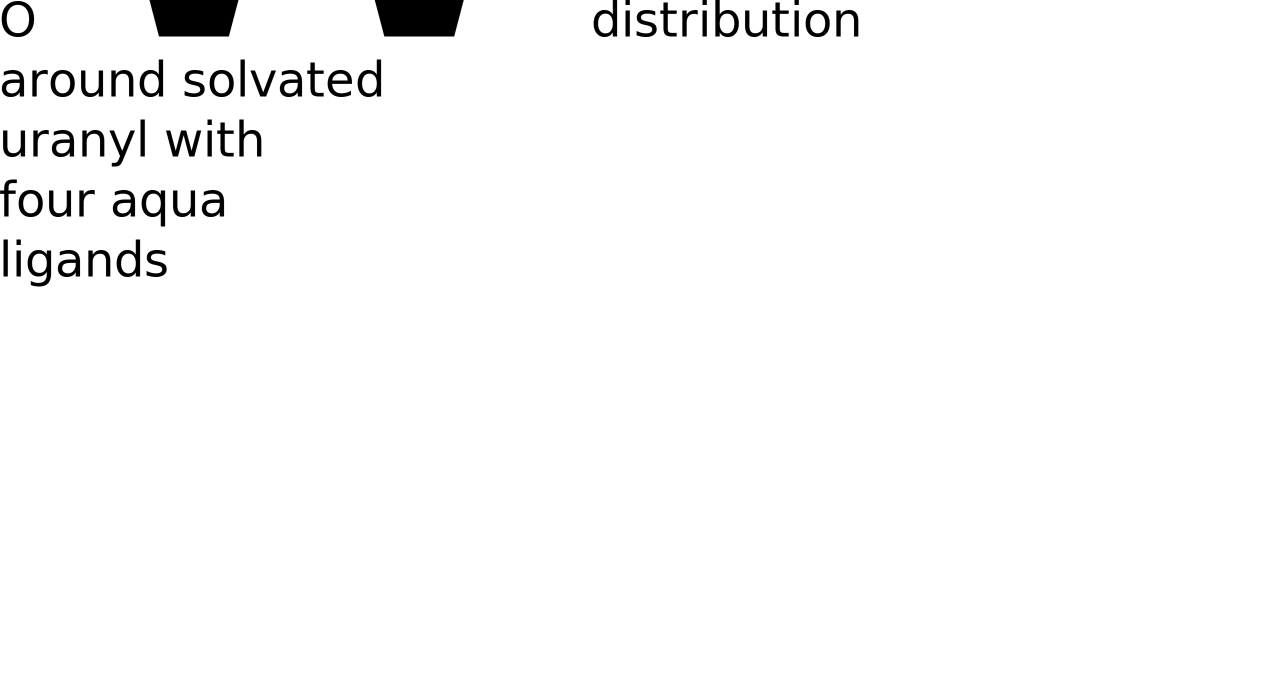
\includegraphics[height=3.5cm]{toc}
\end{tocentry}
\end{document}
